%%%%%%%%%%%%%%%%%%%%
\newcommand{\functionANHTAO}[2]{
	\functionSignature{\texttt{anhtao-path}}{\varAtomicTask{}{}, \varAgent{}{}}
}

\subsection{Optimising hierarchical task allocation in networks of agents}

To successfully complete a composite task, a sink agent needs to receive composite tasks from an external source, decompose them into atomic tasks, and allocate these to other agents. These agents must choose whether to execute the tasks themselves, utilising their available resources, or allocate them to further agents, extending the task-path.  When sink agents complete a composite task they will then adapt their Q-values to optimise their actions, as well as of those agents on the task-path, given the absolute task values of the completed atomic tasks. To illustrate this, Figure \ref{fig:arc-flow} shows a task-path where there are two re-allocations made before a specific atomic task is allocated to an agent that completes the task by taking a measurement.
\begin{figure}[ht]
	\centering
	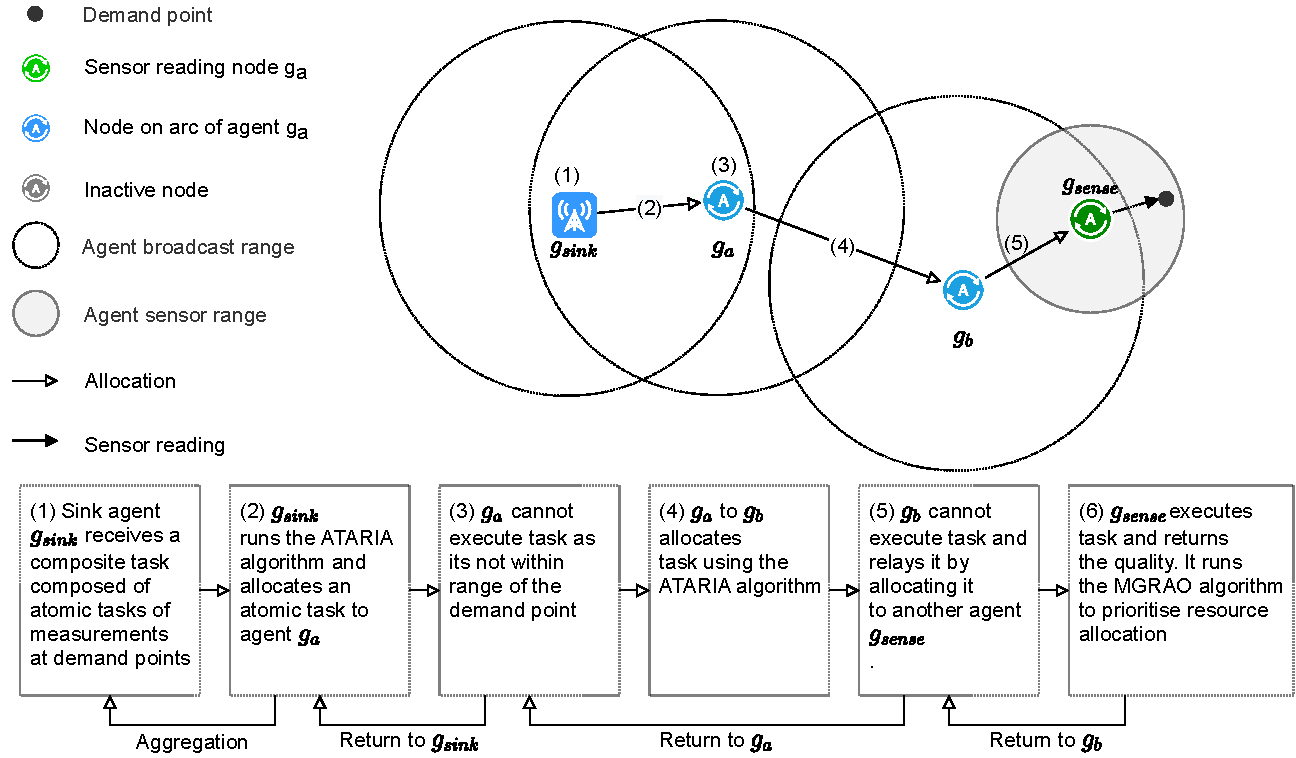
\includegraphics[width=0.8\linewidth, trim={72pt 0pt 62pt 0pt, clip}]{arc-flow}
	\caption{\textbf{Allocation along a task-path}. This diagram illustrates how allocations can be relayed along a task-path using successive applications of the \acronymATARIA{}{} algorithm.}
	\label{fig:arc-flow}
\end{figure}
The high-level flowchart in Figure \ref{fig:algorithm-flow}(a) shows how sink node agents decompose composite tasks, choose actions to take, allocate atomic tasks, and return results. In Figure \ref{fig:algorithm-flow}(b) we can see how agents in a task-path choose actions, and how they execute or re-allocate the atomic tasks they have been allocated.

\begin{figure}[ht]
	\centering
	\begin{subfigure}{.49\textwidth}
		\centering
		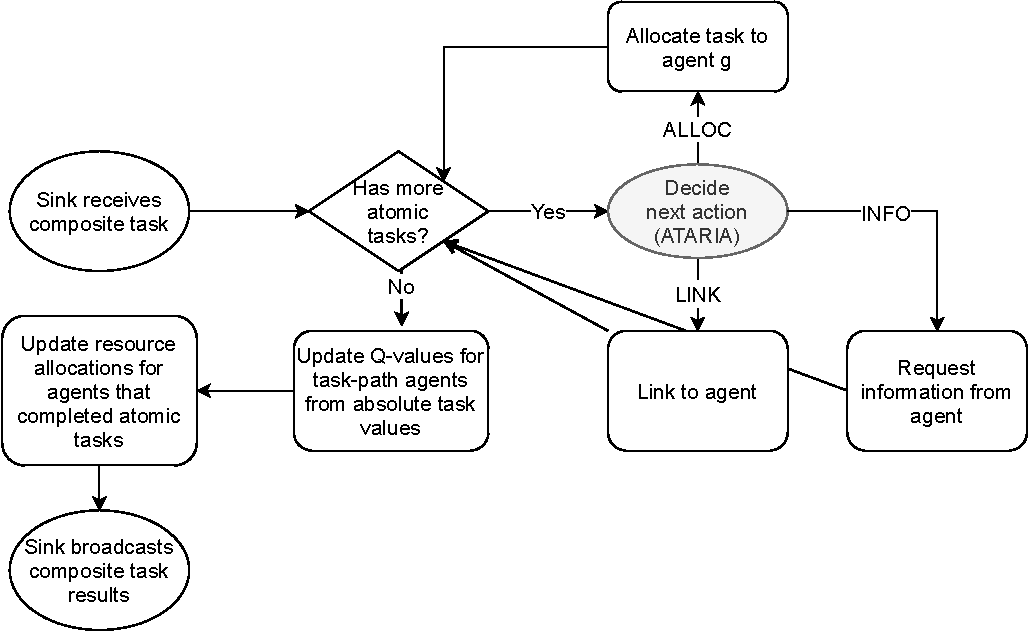
\includegraphics[width=0.9\linewidth, trim={25pt 0pt 25pt 0pt, clip}]{algorithm-flow-sink}
		\caption{Sink agent flow}
		\label{fig:algorithm-flow-sink}
	\end{subfigure} \hfill%
	\begin{subfigure}{.49\textwidth}
		\centering	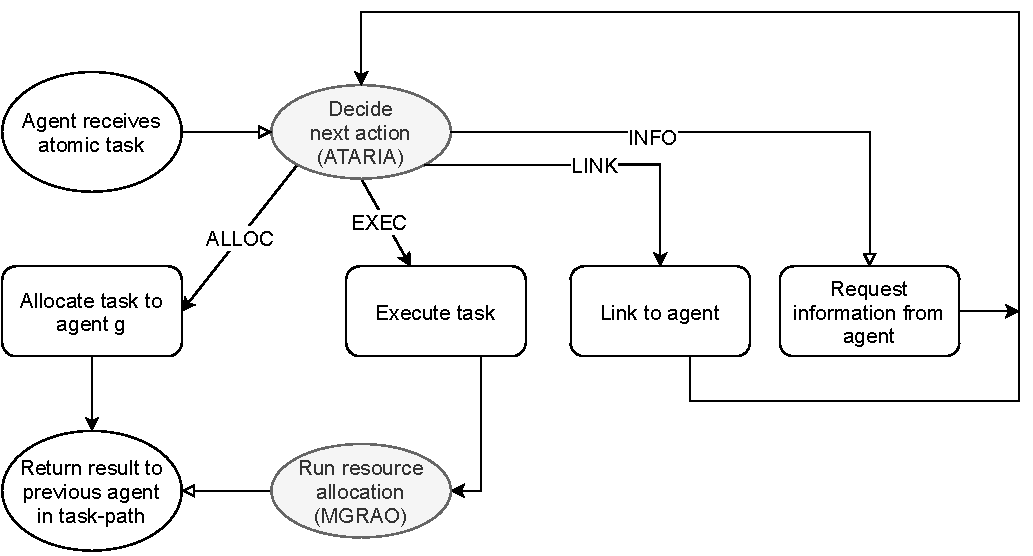
\includegraphics[width=0.9\linewidth,trim={25pt 0pt 25pt 0pt, clip}]{algorithm-flow-arc}
		\caption{Task-path agent flow}
		\label{fig:algorithm-flow-arc}
	\end{subfigure}
	\caption{\textbf{\acronymWSNOptimisation{}{} execution flowchart.} Shows how \acronymWSNOptimisation{}{} combines the \acronymATARIA{}{} and \acronymMGRAO{}{} algorithms and enables recursive allocation of tasks.}
	\label{fig:algorithm-flow}
\end{figure}